\chapter{Evaluation and Results}
%Here you can see a citation: \cite{atc13}.
%\lipsum[7]
In this chapter, we present the evaluation procedure employed as well as the results obtained for the three datasets that were used in our experiments.

\section{Dataset-I}
As mentioned earlier, the Urban8K dataset has one audio class per audio recording which makes it a candidate database for a monophonic audio even detection system. Table~\ref{tab:db1} reviews all the audio classes present in this dataset. 

\begin{table}[tb]
\caption[Urban8K Dataset]{Urban8K Dataset}
\label{tab:db1}
\centering
\begin{tabular}{ccc}
\toprule
Class & ID \\ 
\midrule
air conditioner	& 0 \\
car horn	& 2 \\
children playing	& 3 \\
dog bark	& 4 \\
drilling	& 5 \\
engine idling	& 6 \\
gun shot	& 7 \\
jackhammer	& 8 \\
siren	& 9 \\
street music	& 10 \\
\bottomrule 
\end{tabular}
\end{table}

In the following, we discuss the evaluation procedure that we adopted to evaluate our results and then we present the results of our models trained on this database and compare those results with the baseline results available from the literature.

\subsection{Evaluation Procedure}
Motivated by \cite{salamon2014dataset} which is the source of this dataset, We use the zero-one classification error as the evaluation metric for our results. In the following, we explain how exactly is the zero-one error computed. 

\begin{figure}[tb] 
\centering 
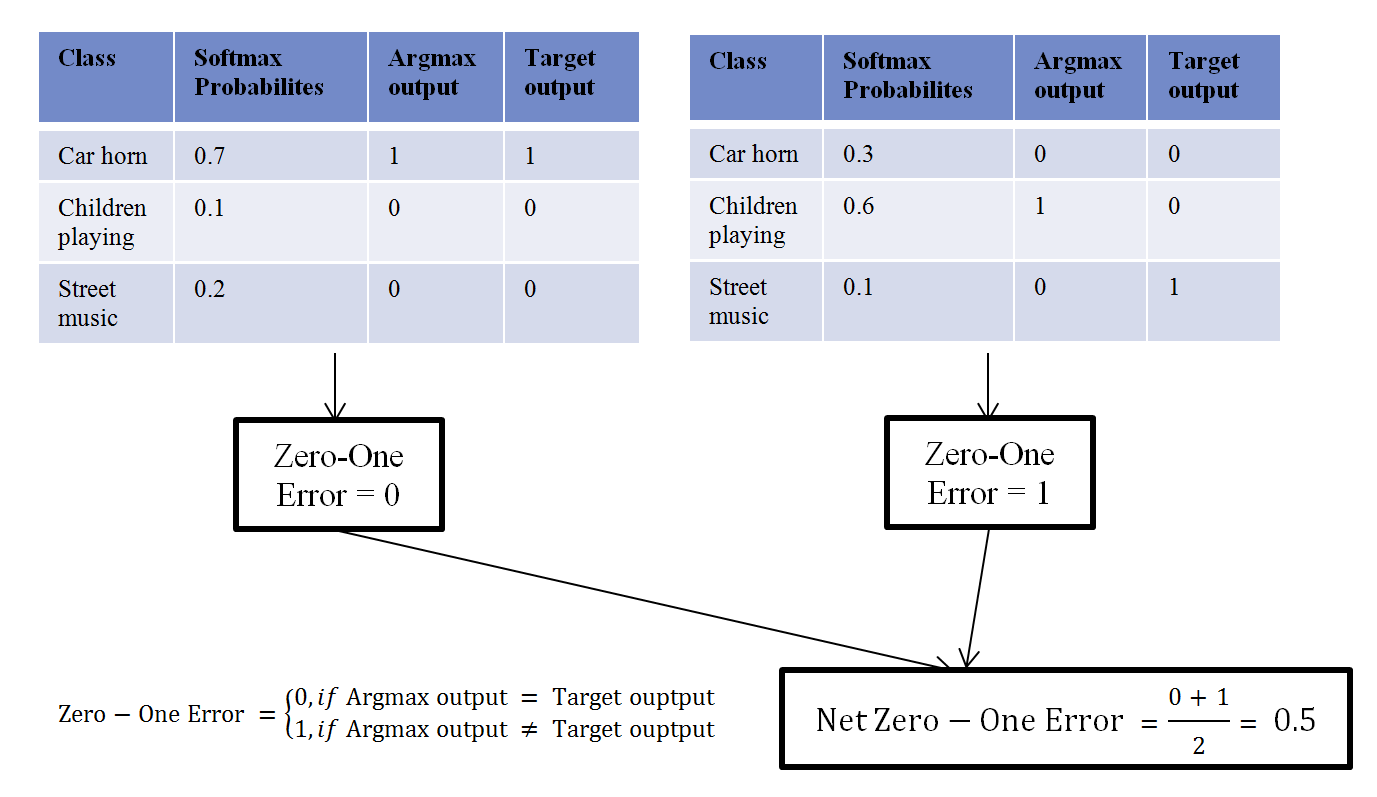
\includegraphics[width=0.9\columnwidth]{eval_schema_db1} 
\caption[Evaluation Schematic]{Evaluation using zero-one error: a schematic}
\label{fig:eval_schema_db1} 
\end{figure}

When the machine learning model is a neural network, as there are 10 classes, the class labels or the ground truth for each of the 10 classes is first converted to one-hot\footnote{one-hot vectors are binary vectors consisting of 0's and 1's with a single non-zero element} vectors of size 10. For example, a recording labeled as "air conditioner''  (i.e. ID = 0) will translate to the one-hot vector [1 0 0 0 0 0 0 0 0 0], another one labeled as "dog bark'' (ID = 4) would be written as [0 0 0 0 1 0 0 0 0 0], and so on. Similar to the ground truth, the predictions made by the machine learning models are also vectors of size 10. But, instead of 0's and 1's, these vectors consists of probabilities. For example, if we have a prediction vector [p$_{\text{1}}$ p$_{\text{2}}$ p$_{\text{3}}$ p$_{\text{4}}$ p$_{\text{5}}$ p$_{\text{6}}$ p$_{\text{7}}$ p$_{\text{8}}$ p$_{\text{9}}$ p$_{\text{10}}$] for a certain audio recording, then p$_{\text{1}}$ indicates the probability of this audio recording being an air-conditioner sound, p$_{\text{2}}$ for a car-horn sound and so on. When the machine learning model outputs these probability vectors, they are passed through the softmax function, so that all the 10 probabilities inside the vector sum to 1.

As we have both the ground truth and the prediction, they can now be compared to obtain the error. If the argmax of the prediction vector equals to the argmax of the ground truth vector, then the error is zero, else the error is one. This error is the error for one audio recording. The final error is simply the average of all such errors over all the audio recordings that are being used for testing/evaluation. Figure~\ref{fig:eval_schema_db1} shows a simplified schematic of the evaluation procedure for a toy dataset of 2 audio recordings with 3 audio classes.

\begin{figure}[!htb] 
\centering 
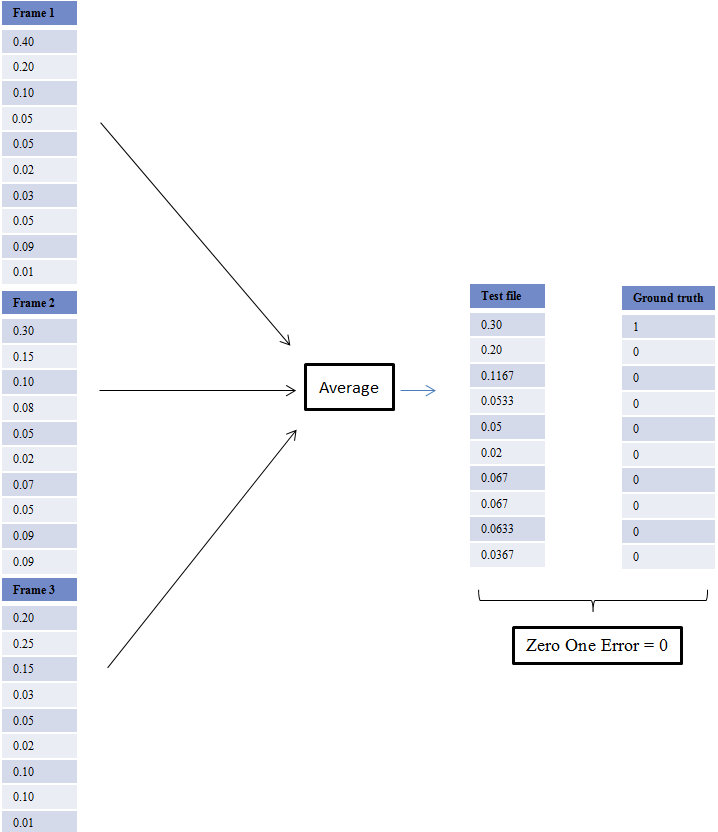
\includegraphics[width=0.95\columnwidth]{post_process_schema_db1} 
\caption[Post processing Schematic]{Evaluation by averaging the frame-wise predictions: a schematic}
\label{fig:post_process_schema_db1} 
\end{figure}

For the above case, one audio recording means one training instance for the machine learning model. That is, one audio recording is labeled by a 10-size vector. There is another possibility, where one audio recording is broken down into individual frames, and then each frame becomes one training instance. In this case one audio recording still has a single ground-truth label vector, \textsl{n} number of prediction vectors(where n is the number of frames in the recording). In that case, since direct comparison between prediction and ground truth is not possible, we need to process the predictions. This is called the pre-processing step, where we either (i)average the probabilities for each of the 10 classes across all the frames and this averaged prediction vector, or (ii)decide the argmax of the predictions on the basis of majority voting i.e. pick that class as the predicted output which has the highest probability in a majority of frames. Both approaches (i) and (ii) are commonly used in literature but we have used approach (i) wherever applicable, primarily because it was easier to use. Figure~\ref{fig:post_process_schema_db1} shows a schematic consisting of the predictions from 3 frames, which are averaged and then compared to the ground truth.

For machine learning models other than artificial neural networks, like the support vector machines or k-nearest neighbors, we do not need to convert the class labels into one-hot vectors. Instead we can use the class IDs (as shown in table~\ref{tab:db1}) as class labels for each of the 10 classes. Nonetheless, the evaluation metric remains the same i.e. the zero-one classification error. If the predicted label matches the ground truth label, then the error is zero, else one. Once again, we take the average of all the zero-one errors of all the audio recordings to calculate the final error. Notice that there is no need to calculate argmax in this way of calculating error.

Finally, apart from obtaining the zero-one classification error, we also measure the confusion matrix, which is a 10X10 matrix in this case (10 is the number of audio classes). Confusion matrix gives us an idea of the class-wise classification accuracy of the model/classifier. The class-wise performance of the can not be gauged from the zero-one classification error. Using confusion matrix, we can identify which classes in particular are the most difficult/easy to be classified or which pair of classes are confused the most often, etc.


\subsection{Results}

\subsubsection{Baseline: k-Nearest Neighbors}

\begin{figure}[!htb] 
\centering 
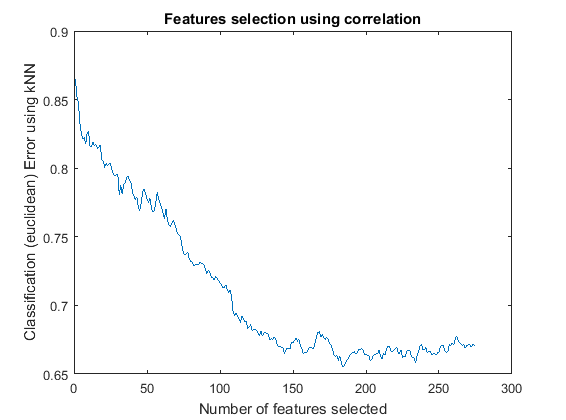
\includegraphics[width=0.8\columnwidth]{feature_selection_using_correlation} 
\caption[Feature Selection]{Feature Selection Using Correlation}
\label{fig:feature_selection_using_correlation} 
\end{figure}


\begin{figure}[!htb] 
\centering 
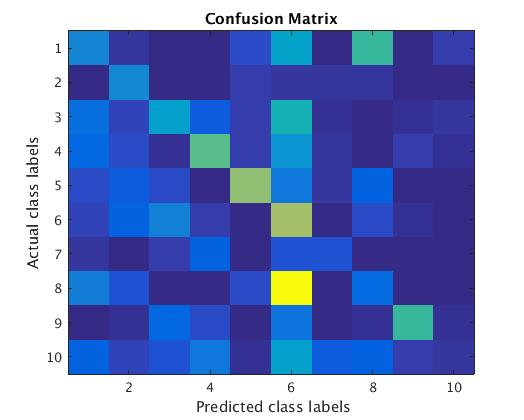
\includegraphics[width=0.8\columnwidth]{kNN_conf_mat} 
\caption[kNN Confusion Matrix]{Confusion Matrix for the kNN model}
\label{fig:kNN_conf_mat} 
\end{figure}

\begin{figure}[!htb] 
\centering 
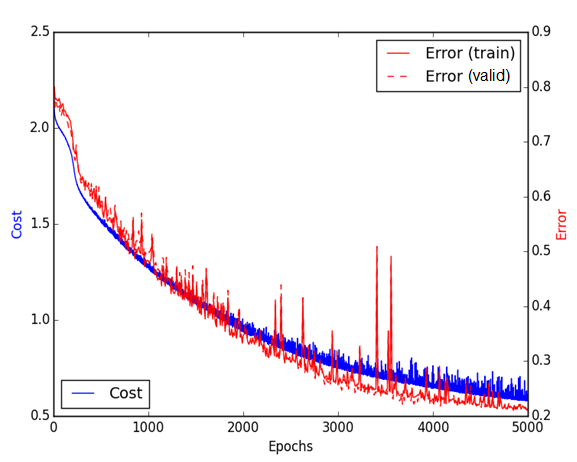
\includegraphics[width=0.8\columnwidth]{dnn_learning_curve_db1} 
\caption[DNN Learning Curve]{Learning Curve for the DNN training}
\label{fig:dnn_learning_curve_db1} 
\end{figure}

In an attempt to reproduce the kNN results published in \cite{salamon2014dataset}, we implemented a kNN(k=5) model in MATLAB and performed a 10-fold cross validation experiment. Euclidean distance was used as the distance/error metric for computing the errors in the kNN model We obtained average classification accuracy of 33.4\%. However the result published in the paper is 56\%. Upon contacting the authors, we learned that they have used an additional attribute selection process, which is tersely mentioned in the paper. We tried to follow the described attribute selection procedure by the authors that says - those features should be chosen which have a high correlation with the output and low correlation with other features. Upon trying to keep the top \textsl{k} features (k varies from 1 to 275, where 275 is the size of the feature vector in our experiments) based on correlation, and evaluating the classification errors using the kNN model, we obtained the zero-one classification errors as shown in figure~\ref{fig:feature_selection_using_correlation}. By using attribute selection based on correlation, we achieve the best classification accuracy of approximately 35\%, which is still far from the paper's results. 

Hence, we could not reproduce the results even by following the attribute selection step performed by the authors. We tried to further contact the authors and received no further reply. At this point, we discontinued to work further on the kNN model for this dataset. Figure~\ref{fig:kNN_conf_mat} shows the confusion matrix obtained using the kNN model. In the figure, class labels are labeled from 1 to 10 instead of 0 to 9. Blue color represents smaller values and yellow color represents higher values in the matrix (dark blue would mean a value close to zero). It can be noticed that there is a noticeably high confusion between classes 'Engine Idling' and 'Jackhammer'. Overall, there are lots of confusions between the audio classes, which is evident by a lot of non-zero non-diagonal entries. We treat these results as our baseline results. Note that a random classifier would have an accuracy of 10\% for this dataset because we have 10 uniformly distributed audio classes. Hence, the kNN model at least performs significantly better than a random classifier.

\begin{table}[tb]
\caption[DNN Hyperparamters DB1]{Hyper-parameter setting for the DNN model}
\label{tab:dnn_hyper_db1}
\centering
\begin{tabular}{ccc}
\toprule
Hyper-parameter & Value \\ 
\midrule
Feature type	& MFCCs, delta MFCCs, delta-delta MFCCs \\
Size of input feature vector	& 150 \\
Number of hidden layer	& 5 \\
Number of hidden neurons in each layer	& Sigmoid \\
Number of neurons(units) used in output layer	& 10 \\
Activation function for output layer	& Sigmoid \\
Learning rate for training	& 0.1 \\
Learning rate for pre-training	& 0.5 \\
Pre-training type & Auto-encoder \\
Number of epochs for training	& 5000 \\
Number of epochs for pre-training	& 300 \\
Batch size for pre-training and training	& 100 \\
Number of training data samples	& 5700 \\
Number of validation data samples	& 1200 \\
Cost function for training	& Categorical cross entropy \\
Cost function for pre-training & L$_{\text{2}}$ squared error\\
Error metric for training and validation	& Zero-one classification error\\
\bottomrule 
\end{tabular}
\end{table}

\subsubsection{Deep Neural Network}
The hyper-parameters used for the network are primarily derived from \cite{gencoglu2014recognition} and then modified on the basis of experiments that we conducted for fine-tuning the network. A review of all the hyper-parameters is presented in table~\ref{tab:dnn_hyper_db1}. Figure~\ref{fig:dnn_learning_curve_db1} displays the learning curve that shows the cost function, training and validation errors obtained by training the network for 5000 epochs.

By training the DNN with this hyper-parameter setting and subsequently testing on the test data, we obtained a classification accuracy of 40.8\%. This is better than the best result obtained from our kNN model but still far poorer than the best achieved accuracy of around 68\% on this dataset in the literature. One reason for obtaining poorer results is the missing attribute selection step in our work that has been used in the literature. Another reason is a limitation in our DNN model because we have compressed the frame-wise information of an audio recording into a single vector by taking the average and standard deviation of the feature vectors of all the frames. This compression leads to loss of information especially the contextual knowledge that flows between consequent frames. Furthermore, we have approximately 5700 training instances which is relatively small amount of data to train a deep neural network, and this could be another reason of such performance of the DNN.

\begin{figure}[!htb] 
\centering 
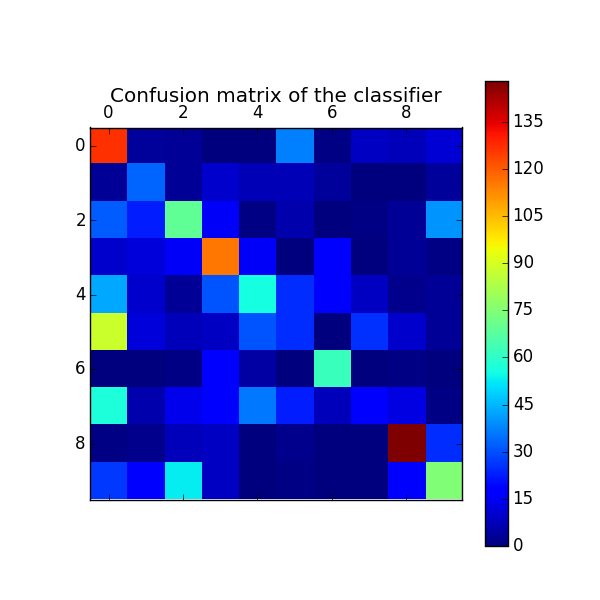
\includegraphics[width=0.8\columnwidth]{dnn_conf_mat_db1} 
\caption[Confusion Matrix DNN]{Confusion Matrix of the DNN model}
\label{fig:dnn_conf_mat_db1} 
\end{figure}

In addition to the classification accuracy, we also obtained the confusion matrix for our DNN classifier which is shown in figure~\ref{fig:dnn_conf_mat_db1}. First, it can be noticed from the figure that audio class 'Siren' has the highest classification accuracy. This could be because of the high distinctiveness of a siren sound from the other audio classes such that the spectral features for this class are very different. Secondly, many of the audio recordings seem to be blindly predicted as 'Air Conditioner', and there is a lot of confusion between the classes 'Air Conditioner' and 'Engine Idling'. This indicates that (i)the two classes share a lot of common spectral features that make them hard to be distinguished using our model (they also sound very similar if heard manually), and (ii)'Air Conditioner' sounds are quite 'noise-like' sounds, hence, even for a recording of 'Dog Bark', if there is some noise in the background, it could be misconceived as the 'Air Conditioner' sound. 

Lastly, the audio class 'Gun Shot', although seems to be classified correctly in a majority of times, is not well suited to the frames-compression method that we have used as a pre-processing step in our DNN model. Audio recordings of gun-shots would usually have only a couple of frames (out of hundreds) that actually contain the gun-shot sound, because it happens in merely less than a fraction of a second. Hence, our way of taking the average and standard deviation of feature vectors across all frames is futile for such recordings. Because in our final feature vector, the real information from the frames having the actual features is heavily suppressed by the random noise from all other information-less frames.

\subsubsection{Convolutional Neural Network}

\begin{table}[tb]
\caption[CNN Hyperparamters DB1]{Hyper-parameter setting for the CNN model}
\label{tab:cnn_hyper_db1}
\centering
\begin{tabular}{ccc}
\toprule
Hyper-parameter & Value \\ 
\midrule
Feature type	& MFCCs, delta MFCCs, delta-delta MFCCs \\
Number of input feature maps	& 74 \\
Number of output feature maps	& 10 \\
Number of convolutional layers	& 1 \\
Number of pooling layers	& 1 \\
Number of hidden/affine layers	& 1 \\
Pooling type	& Max-pooling \\
Kernel Size	& (3X1) \\
Activation function for the hidden and output layers & Sigmoid\\
Number of units/neurons in the output layer	& 10 \\
Learning Rate for training	& 0.0003 \\
Number of epochs of training	& 1000 \\
Batch size	& 50 \\
Number of training data samples	& 4500 \\
Number of validation data samples & 1200 \\
Cost function for training	& Categorical cross entropy \\
Error metric for training and validation	& Zero-one classification error\\
\bottomrule 
\end{tabular}
\end{table}

To be able to capture the spectral information across the frames of an audio recording without having to simply summarize the information of all frames by averaging, we use a CNN model with the motivation of capturing the sequential changes in information by the way of obtaining gradients in a convolution operation. We started with a simple CNN model setting and then finalized the hyper-parameters on the basis of conducted experiments with various hyper-parameter settings for fine-tuning the network. A review of all the hyper-parameters is presented in table~\ref{tab:cnn_hyper_db1}.

\begin{figure}[!htb] 
\centering 
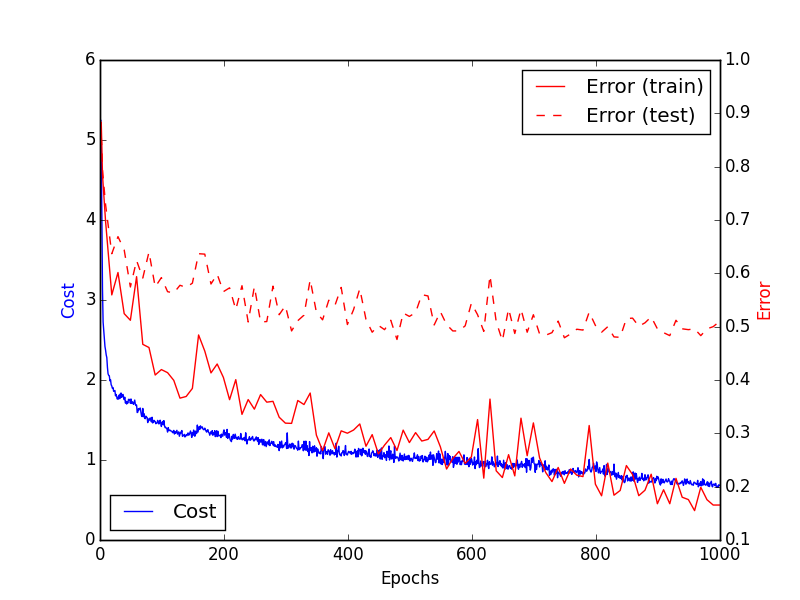
\includegraphics[width=0.8\columnwidth]{learning_curve_cnn_db1} 
\caption[Learning Curve CNN]{Learning Curve of the CNN model}
\label{fig:learning_curve_cnn_db1} 
\end{figure}

The learning curve, with the cost function, training and validation errors for the 1000 epochs of training is shown in figure~\ref{fig:learning_curve_cnn_db1}. From the learning curve it is evident that as the epochs progress, the model tends to fit better to the training data but the model performance on the validation data stagnates after a certain number of epochs.

We obtain a zero-one classification accuracy of 52.51\% by testing the trained CNN model on the validation set. This result is much better than the previous two models - kNN and DNN. An explanation for this could be that in the CNN model, (i)we are somewhat able to keep the contextual information across the frames of an audio recording by performing the convolution step, and (ii)we are extracting the most useful information from each audio recording by performing the max pooling step contrary to just taking the average of information from all frames in the DNN model. 

\begin{figure}[!htb] 
\centering 
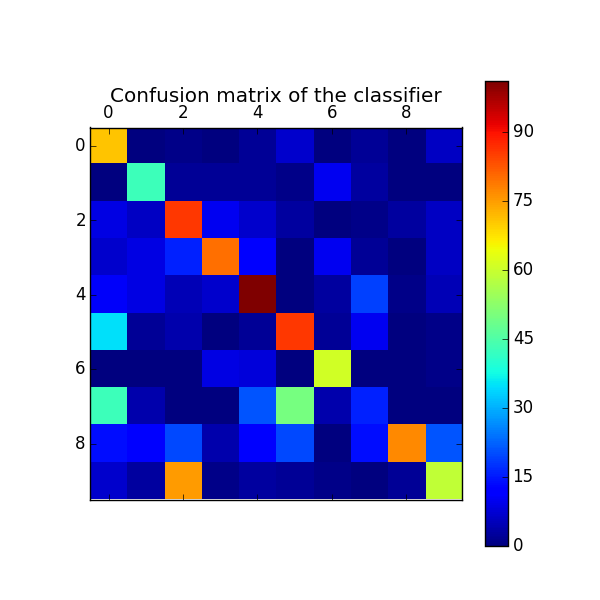
\includegraphics[width=0.8\columnwidth]{cnn_conf_mat_db1} 
\caption[Confusion Matrix CNN]{Confusion Matrix of the CNN model}
\label{fig:cnn_conf_mat_db1} 
\end{figure}

Figure~\ref{fig:cnn_conf_mat_db1} shows the confusion matrix for this model. First it can be noticed from the matrix that the audio class 'Drilling' has the highest classification accuracy, which indicates that drilling sound is the easiest and the most distinctive to be classified by CNN model. Secondly, as noticed for the DNN model, many of the audio recordings are blindly predicted as 'Air Conditioner', and there is a lot of confusion between the following pairs of audio classes: (i)'Engine Idling' and 'Air Conditioner', (ii)'Jackhammer' and 'Air Conditioner', (iii)'Jackhammer' and 'Engine Idling', and (iv)'Children Playing' and Street Music'. Pairs (i) and (iv) have also been reported to be confusing in relevant literature and would probably also sound confusing when heard manually. And the confusion in pairs (ii) and (iii) could be due to the way the CNN extracts features. Lastly, the audio class 'Jackhammer' is classified correctly for the least number of times. Most of the actual jackhammer sounds are being incorrectly classified as 'Air Conditioner' or 'Engine Idling'. As this was not observed with the previous two models, this phenomenon could be reasoned as a result of the convolution and/or max-pooling operation.

Figure [...........] presents a comparison of our results from the three different models along with the results from the literature. As stated earlier, we do not reach the best literature results which is primarily due to a missing attribute selection step in our work. However, it can be reasoned that considering our kNN model, which is an attempt to reproduce the baseline results from the literature as our baseline, we have improved the classification accuracy significantly by using the CNN model. With the additional attribute selection step, the accuracy of the CNN model might further improve. However, in the absence of any further knowledge about the exact attribute selection procedure employed in \cite{salamon2014dataset}, we discontinued our research on this dataset at this point.


\section{Dataset-II}
As mentioned earlier, the Freesound dataset is composed of a selection of publicly available audio recordings at \url{www.freesound.org} which are annotated by the authors of \cite{kons2013audio}. It has six potentially overlapping audio classes, which makes it a database suitable for a polyphonic audio event detection system. 

Despite of the six available classes, \cite{kons2013audio} has published its baseline results using only the four classes: (i)Crowd, (ii)Applause, (iii), Music, and (iv)Traffic. For consistency, we also worked only with these 4 classes. In all our machine learning models, we trained 4 different one-vs-all binary classifiers for the 4 audio classes. In the end, we averaged the results obtained from the 4 binary classifiers to get the final result. This approach of using 4 different binary classifiers instead of one multi-class classifier provides us the extra flexibility of fine-tuning the classifier for each class independently as well as better analyze the performance of each classifier individually. However, by following this approach, we neglect the correlation between the occurrences of different audio classes. Table~\ref{tab:db2} presents a review of the four classes along with the total length of the recordings that belong to each of these classes. 

\begin{table}[tb]
\caption[Freesound dataset]{Freesound Dataset}
\label{tab:db2}
\centering
\begin{tabular}{ccc}
\toprule
Audio Class & Length (in minutes) \\ 
\midrule
Crowd	& 45.625 \\
Applause	& 26.958 \\
Music	& 27.625 \\
Traffic	& 34.375 \\
\bottomrule 
\end{tabular}
\end{table}

In the following, we discuss the evaluation procedure that we adopted to evaluate our results and then we present the results of our models trained on this database and compare those results with the baseline results available from the literature.

\subsection{Evaluation Procedure} \label{eval_proc_db2}
Motivated by \cite{kons2013audio} which is the source of this dataset, we use the equal error rate as the evaluation metric for our results. In the following, we explain how exactly is the EER computed. 

Calculating equal error rate on the receiver operator characteristics (ROC) curve \cite{bradley1997use} is a reliable way of estimating classification accuracy in the case of binary classification problems with a major class-skew. In our case in each of the 4 binary classifiers, the number of positive samples is much smaller than the number of negative samples, which means a class skew. This justifies the use of EER as the error metric in this case.

\begin{figure}[!htb] 
\centering 
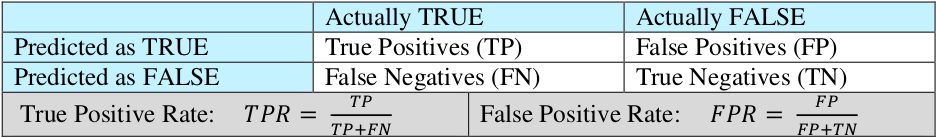
\includegraphics[width=0.8\columnwidth]{tpr_fpr} 
\caption[TPR-FPR]{TPR and FPR}
\label{fig:tpr_fpr} 
\end{figure}

\begin{figure}[!htb] 
\centering 
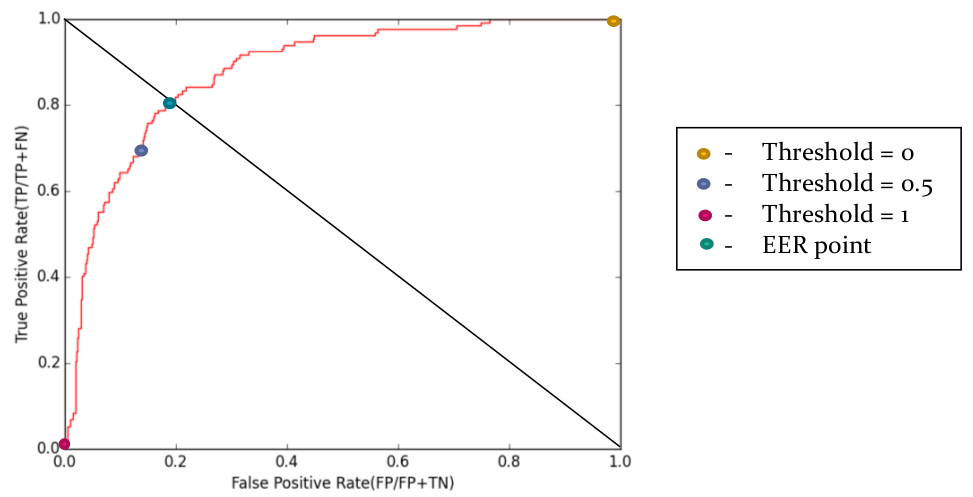
\includegraphics[width=0.8\columnwidth]{roc_eer} 
\caption[ROC-EER]{ROC Curve and EER}
\label{fig:roc_eer} 
\end{figure}

In the dataset, the audio recordings are 5 seconds long. For each audio recording and for each binary classifier, a probability is predicted which is then compared to the ground truth binary label (0 or 1). For comparison, the predicted probability has to be converted to a binary number (0 or 1). This is done by thresholding the probability. For example, if the threshold is kept at 0.5, then if the prediction is greater than or equal to 0.5 (eg 0.7), the thresholded prediction would be 1, else the thresholded prediction would be 0. The ROC curve is plotted between the \textsl{true positive rate (TPR)} and the \textsl{false positive rate (FPR)} by varying the threshold from 0 to 1. Figure~\ref{fig:tpr_fpr} gives a summary about the TPR and FPR in binary classification. Figure~\ref{fig:roc_eer} demonstrates a sample ROC curve and the EER point on that curve. EER is defined as the point on the ROC curve where the false rejection rate (1-TPR) equals the false acceptance rate (FPR). When performing k-folds cross validation, we provide the Standard Error (SE) along with the EER, where SE is the standard deviation in EER divided by the square root of k.

\subsection{Results}

\subsubsection{Baseline: Support Vector Machine}
SVM model parameters are mainly derived from \cite{kons2013audio}. We used an RBF kernel function (with $\gamma=0.2$). We trained 4 different one-vs-all binary classifiers for the 4 classes: (i)Crowd, (ii)Applause, (iii), Music, and (iv)Traffic. We considered those audio recordings as the positive data samples for an audio class, which have at least one of its frames belonging to that audio class. Using EER along with SE as the error metric, we performed a 50-fold hold-out cross validation experiment with roughly 80\% of training data and 20\% of validation data. 

Some of the audio recordings which belonged to 'Music' class in the original dataset used in ~\cite{kons2013audio}, are no more available. Hence we compensated for this by manually adding a proportionate length of randomly chosen musical recordings from the same website \footnote{\url{www.freesound.org}}. We obtained the results from our SVM model both with and without the externally added 'Music' audio recordings. The results are shown in table~\ref{tab:svm_db2}, where the error is represented as $EER \pm SE$. The overall results are calculated by simply averaging the EER and SE across all the 4 classes.

\begin{table}[tb]
\caption[SVM Results DB2]{SVM class-wise as well as overall results (EER)}
\label{tab:svm_db2}
\centering
\begin{tabular}{cccc}
\toprule
Audio Class & SVM  & SVM & SVM  \\
& (results from \cite{kons2013audio}) & (our results without compensation) & (with compensation) \\
\midrule
Crowd	& $19.82 \pm 1.15$ & $17.78 \pm 1.19$ & $17.45 \pm 1.08$ \\
Applause	& $10.18 \pm 0.81$ & $12.49 \pm 0.82$ & $12.87 \pm 1.07$ \\
Music	& $17.77 \pm 1.15$ & $37.83 \pm 1.89$ & $23.82 \pm 1.82$  \\
Traffic	& $16.38 \pm 0.77$ & $15.69 \pm 1.13$ & $16.88 \pm 1.22$  \\
\bottomrule 
\end{tabular}
\end{table}

\subsubsection{1-D Convolutional Neural Network} \label{cnn_results_db2}
Similar to the SVM model, we have 4 different CNN models for the 4 classes, each model being a binary classifier. A review of all the selected hyper-parameters for the CNN is shown in table~\ref{tab:1d_cnn_hyper_db2}. All the 4 CNN models are trained with the same set of hyper-parameters except that for the 'Applause' model, CNN is trained for 500 epochs as it learned quicker compared to the other class models. We performed a 50-fold hold-out cross validation experiment with roughly 80\% of training data and 20\% of validation data.

The cost function used is a modified cross-entropy function to account for the skew in the amount of data in the positive and negative classes. We call it a weighted binary cross entropy function and its idea is derived from \cite{kons2013audio}. The formula for this error metric along with the weights used in the case of each class are shown in figure~\ref{fig:w_b_c_e}. The weights of the classes are inversely proportional to the size of the respective class. In the following we discuss the results of each of the 4 models starting with 'Crowd', followed by the overall (averaged) results.

\begin{figure}[!hb] 
\centering 
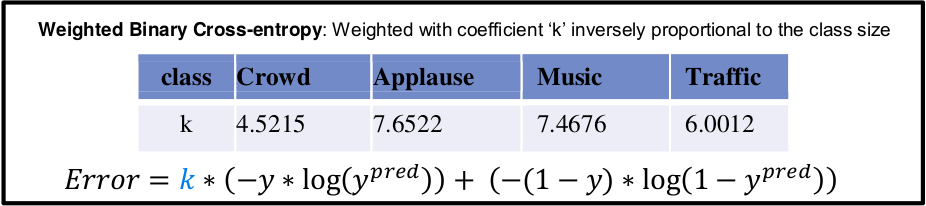
\includegraphics[width=0.9\columnwidth]{w_b_c_e} 
\caption[Weighted Binary Cross-Entropy]{Weighted Binary Cross-Entropy}
\label{fig:w_b_c_e} 
\end{figure}

\begin{table}[tb]
\caption[1-D CNN Hyper-parameters DB2]{Hyper-parameter setting for the 1-D CNN model}
\label{tab:1d_cnn_hyper_db2}
\centering
\begin{tabular}{ccc}
\toprule
Hyper-parameter & Value \\ 
\midrule
Feature type	& MFCCs, delta MFCCs, delta-delta MFCCs \\
Number of input feature maps	& 24 \\
Number of output feature maps	& 4 \\
Number of convolutional layers	& 1 \\
Number of pooling layers	& 1 \\
Number of hidden/affine layers	& 1 \\
Pooling type	& Max-pooling \\
Kernel Size	& (8X1) \\
Activation function for the hidden and output layers & Tanh\\
Number of units/neurons in the output layer	& 1 \\
Learning Rate for training	& 0.003 \\
Number of epochs of training	& 1000 \\
Batch size	& 50 \\
Number of training data samples	& 3800 \\
Number of validation data samples & 800 \\
Cost function for training	& Weighted Binary cross entropy \\
Error metric for training and validation	& Weighted Binary cross entropy\\
\bottomrule 
\end{tabular}
\end{table}



\paragraph{'Crowd' model}
Figure~\ref{fig:crowd_1d_cnn_results} shows the learning curve and the epoch-wise EER error obtained on the train and validation(test) sets for one of the 50 folds. As can be seen from the EER curve, the best EER obtained on the test data is 9.18\%. The learning curve hints towards training the network for more than 1000 epochs, but upon training the same network for 5000 epochs, we obtained the same best EER on the test data as in the case of 1000 epochs.

Figure~\ref{fig:crowd-50CV-noaug} shows the 50-folds cross-validation results for this model. The error for each fold in the figure is the best EER (in \%) obtained on the test data for that fold. We obtain an overall result $(EER \pm SE)$ of $14.86 \pm 0.86$ from the 50 fold cross-validation experiment which is a considerable improvement over the EER of 17.45\% obtained in the SVM model.

\begin{figure}[tb]
\centering
\subfloat[Learning Curve]
{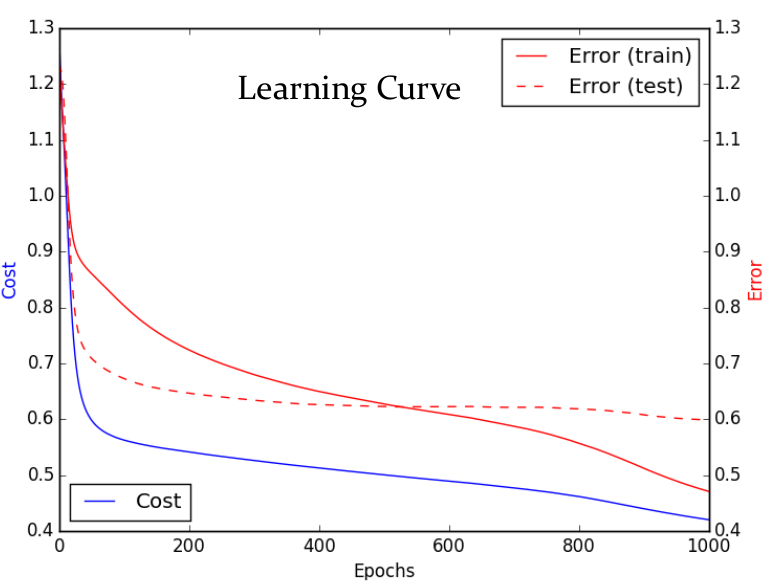
\includegraphics[width=.45\columnwidth]{cnn_crowd_learn_curve}} \quad
\subfloat[EER Curve]
{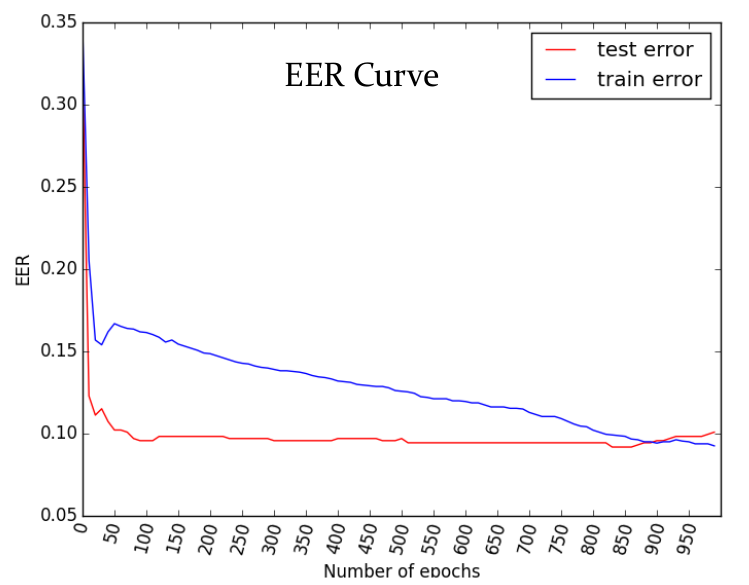
\includegraphics[width=.44\columnwidth]{cnn_crowd_eer_curve}} \\
\caption[Learning Curve and EER Performance of 'Crowd' CNN model]{Learning Curve and EER Performance of 'Crowd' CNN model}
\label{fig:crowd_1d_cnn_results}
\end{figure}

\begin{figure}[!hb] 
\centering 
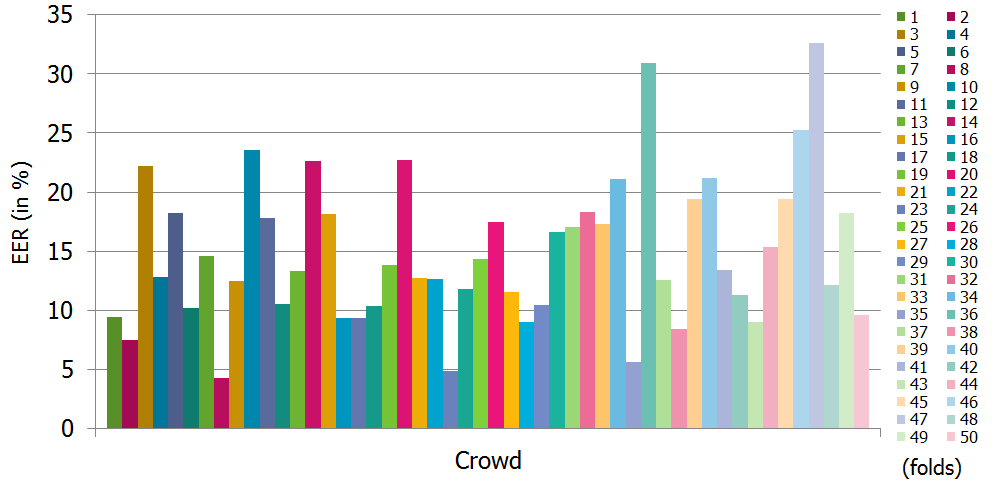
\includegraphics[width=0.9\columnwidth]{crowd-50CV-noaug} 
\caption['Crowd' model: 50-fold cross validation results]{'Crowd' model: 50-fold cross validation results}
\label{fig:crowd-50CV-noaug} 
\end{figure}

\paragraph{'Traffic' Model}
Figure~\ref{fig:traffic_1d_cnn_results} shows the learning curve and the epoch-wise EER error curve obtained upon training the network for one of the 50 folds. From the learning curve, it is evident that after around 200 epochs, the network starts to slightly over-fit the training data. From the EER curve, it can be seen that we obtain the best EER of 15.25\% on the test data for this fold.

Figure~\ref{fig:traffic-50CV-noaug} shows the 50-fold cross-validation results for this model. We obtain an overall result $(EER \pm SE)$ of $11.77 \pm 0.72$, which is much better than the EER of 16.88\% obtained using the SVM model.

\begin{figure}[!hb]
\centering
\subfloat[Learning Curve]
{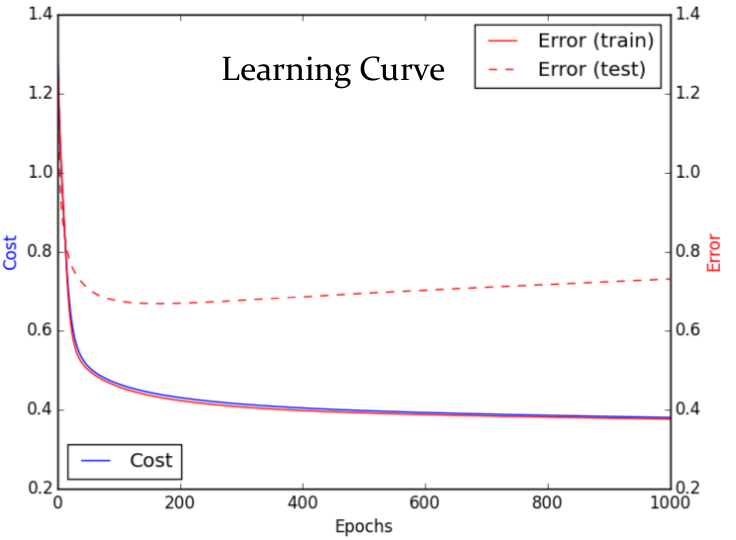
\includegraphics[width=.45\columnwidth]{cnn_traffic_learn_curve}} \quad
\subfloat[EER Curve]
{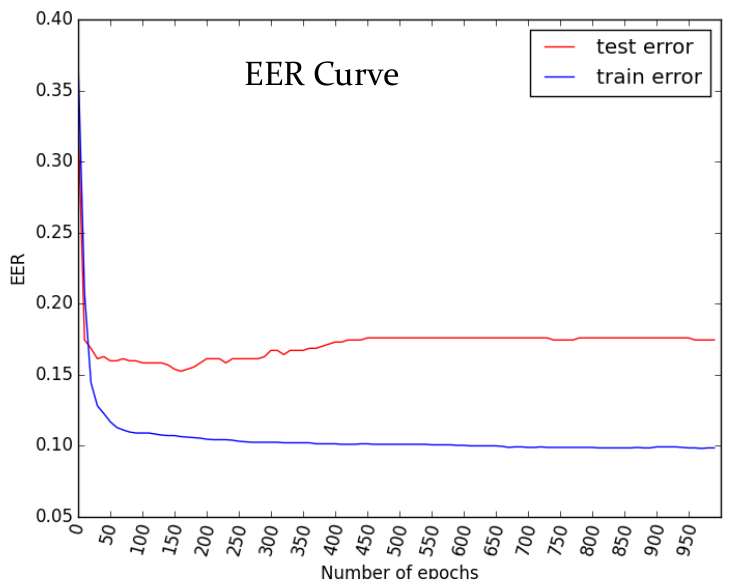
\includegraphics[width=.44\columnwidth]{cnn_traffic_eer_curve}} \\
\caption[Learning Curve and EER Performance of 'Traffic' CNN model]{Learning Curve and EER Performance of 'Traffic' CNN model}
\label{fig:traffic_1d_cnn_results}
\end{figure}

\begin{figure}[!hb] 
\centering 
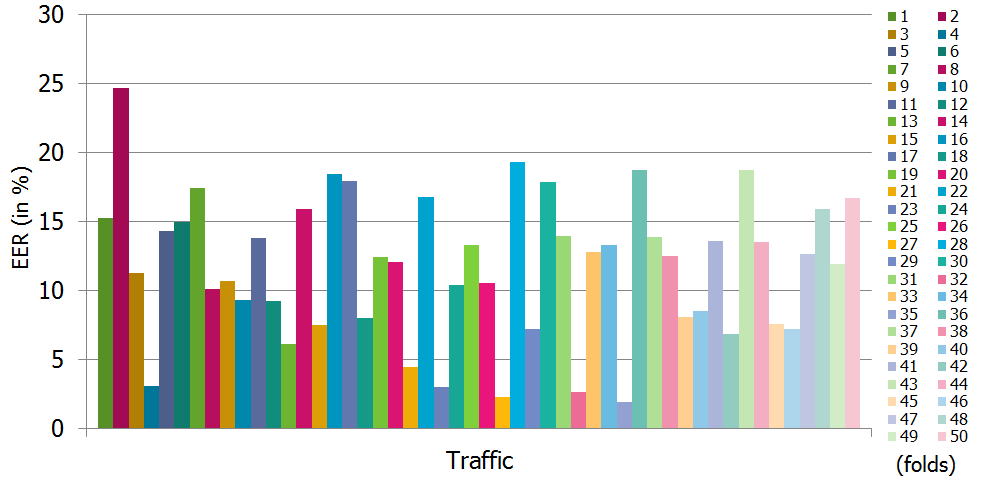
\includegraphics[width=0.9\columnwidth]{traffic-50CV-noaug} 
\caption['Traffic' model: 50-fold cross validation results]{'Traffic' model: 50-fold cross validation results}
\label{fig:traffic-50CV-noaug} 
\end{figure}

\paragraph{'Applause' Model}
As stated earlier, this model is trained only for 500 epochs contrary to 1000 epochs in the case of other models because the CNN model for this class was observed to be quick to train and would generally start heavily overfitting beyond 500 epochs. Figure~\ref{fig:applause_1d_cnn_results} shows the learning curve as well as the EER curve obtained by training the model for one of the 50 folds. From the learning curve it is evident that the network starts overfitting to the training data by the end of 200 epochs. As can be seen from the EER curve, we obtained the best EER of 12.72\% on the test data for this particular fold.

Figure~\ref{fig:applause-50CV-noaug} shows the 50-fold cross-validation results for this model. We obtain an overall result $(EER \pm SE)$ of $4.87 \pm 0.44$, which is much better than the EER of 12.87\% obtained using the SVM model.

%, which is slightly better than the EER of 12.87\% using SVM model. However, our CNN result is poorer than the SVM results from \cite{kons2013audio}. In order to learn more about why this happened, we trained the same CNN model for 'Applause' class, without compensating for the 'Music' recordings, and we obtained an EER of 4.4\%. This implies that our CNN result of 12.72\% EER with the compensated version of dataset is poorer primarily because we are using an altered dataset which is not exactly the same as used in \cite{kons2013audio}.

\begin{figure}[tb]
\centering
\subfloat[Learning Curve]
{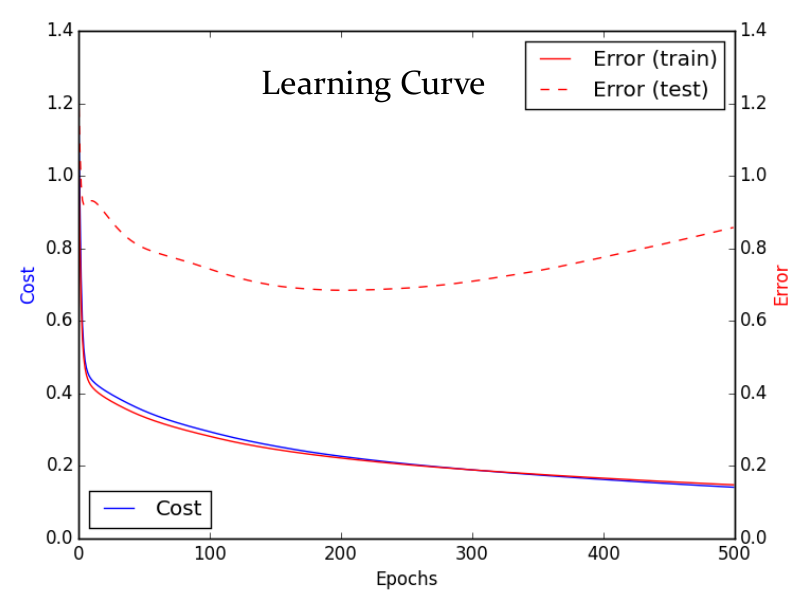
\includegraphics[width=.45\columnwidth]{cnn_applause_learn_curve}} \quad
\subfloat[EER Curve]
{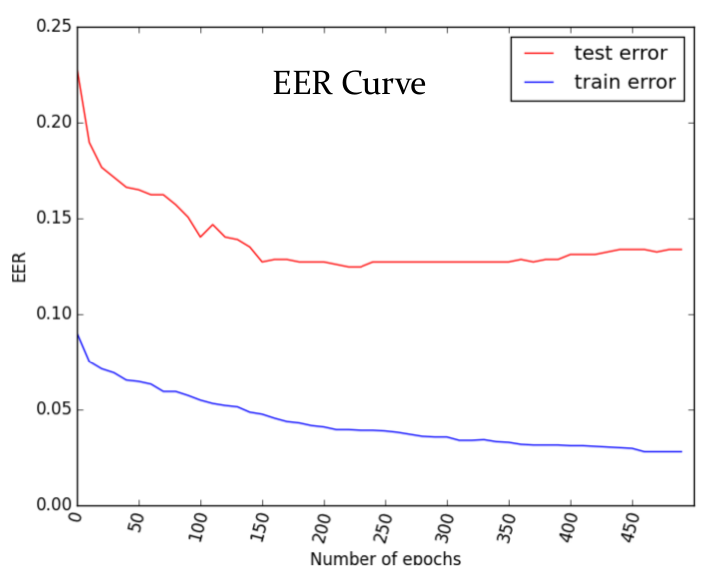
\includegraphics[width=.44\columnwidth]{cnn_applause_eer_curve}} \\
\caption[Learning Curve and EER Performance of 'Applause' CNN model]{Learning Curve and EER Performance of 'Applause' CNN model}
\label{fig:applause_1d_cnn_results}
\end{figure}

\begin{figure}[!hb] 
\centering 
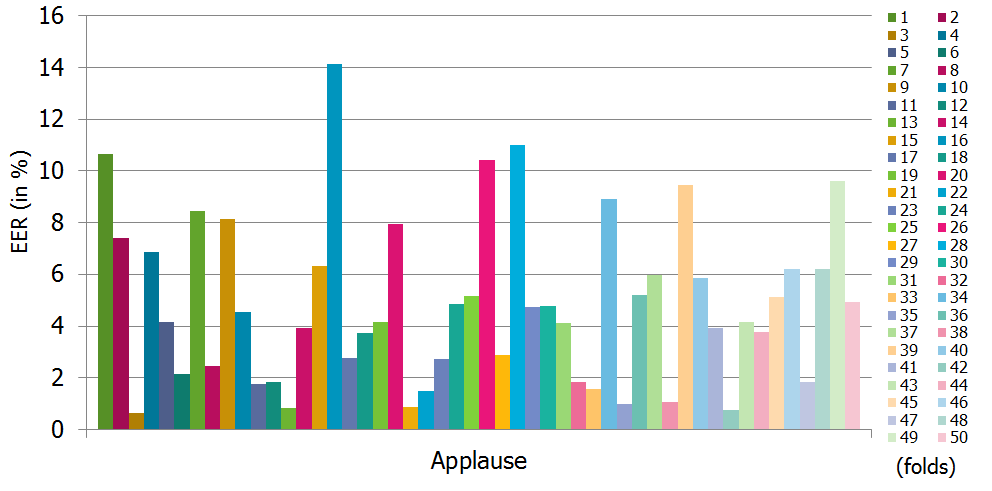
\includegraphics[width=0.9\columnwidth]{applause-50CV-noaug} 
\caption['Applause' model: 50-fold cross validation results]{'Applause' model: 50-fold cross validation results}
\label{fig:applause-50CV-noaug} 
\end{figure}

\begin{figure}[!hb]
\centering
\subfloat[Learning Curve]
{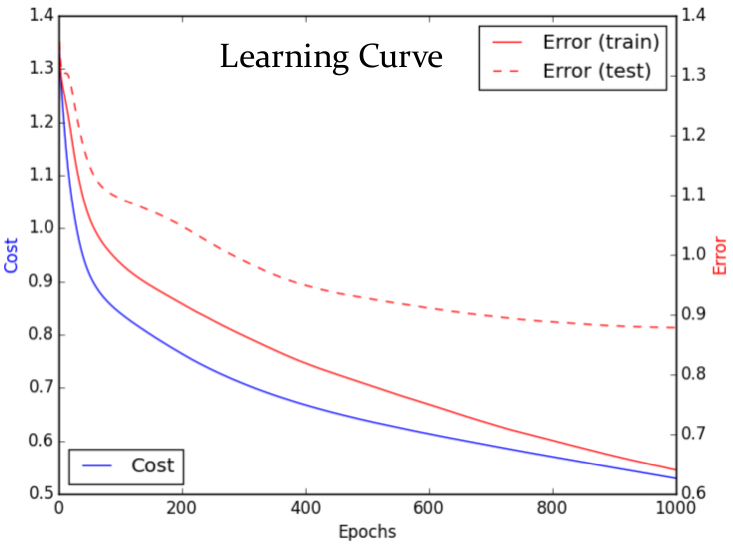
\includegraphics[width=.45\columnwidth]{cnn_music_learn_curve}} \quad
\subfloat[EER Curve]
{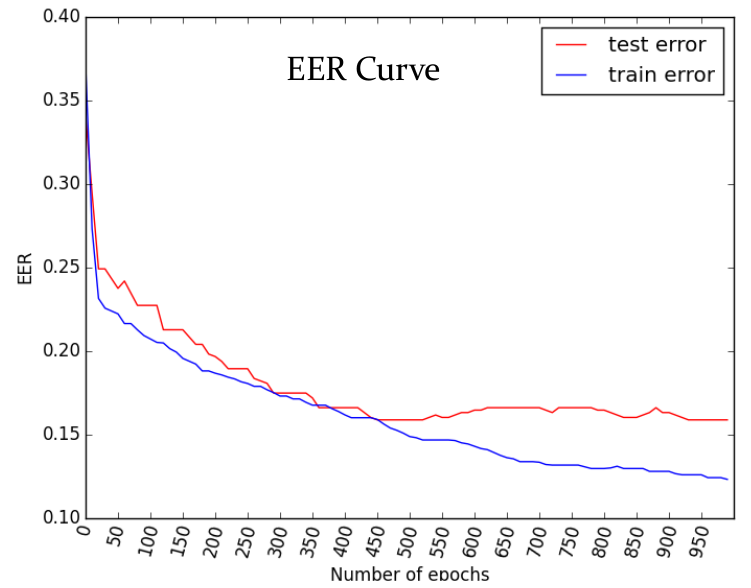
\includegraphics[width=.44\columnwidth]{cnn_music_eer_curve}} \\
\caption[Learning Curve and EER Performance of 'Music' CNN model]{Learning Curve and EER Performance of 'Music' CNN model}
\label{fig:music_1d_cnn_results}
\end{figure}

\paragraph{'Music' Model}
Figure~\ref{fig:music_1d_cnn_results} shows the learning curve and the EER curve obtained by training this CNN model with one of the 50 folds for 1000 epochs. The learning curve clearly indicates that network could be trained for more epochs. Hence, we trained it further for 5000 epochs. Figure~\ref{fig:music_eer_5000} shows the EER curve for 5000 epochs. For this particular fold, we obtained the best EER of 15.89\% when trained until 1000 epochs and the best EER of 15.54\% when trained until 5000 epochs. 

Figure~\ref{fig:music-50CV-noaug} shows the 50-fold cross-validation results for this model. We obtain an overall result $(EER \pm SE)$ of $24.04 \pm 1.23$, which is slightly poorer than the EER of 23.82\% obtained using the SVM model.

\begin{figure}[!htb] 
\centering 
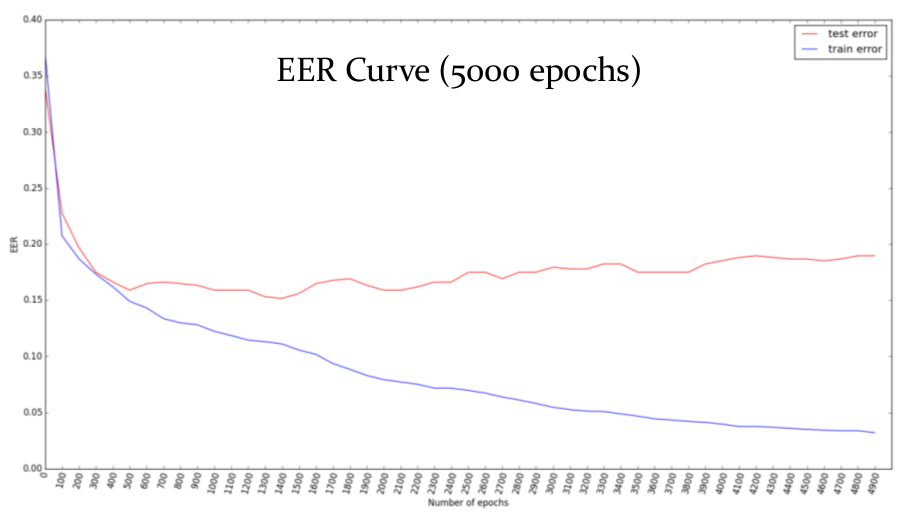
\includegraphics[width=0.95\columnwidth]{cnn_music_eer_curve_5000} 
\caption['Music' model EER curve for 5000 epochs]{'Music' model - EER curve for 5000 epochs}
\label{fig:music_eer_5000} 
\end{figure}

\begin{figure}[!hb] 
\centering 
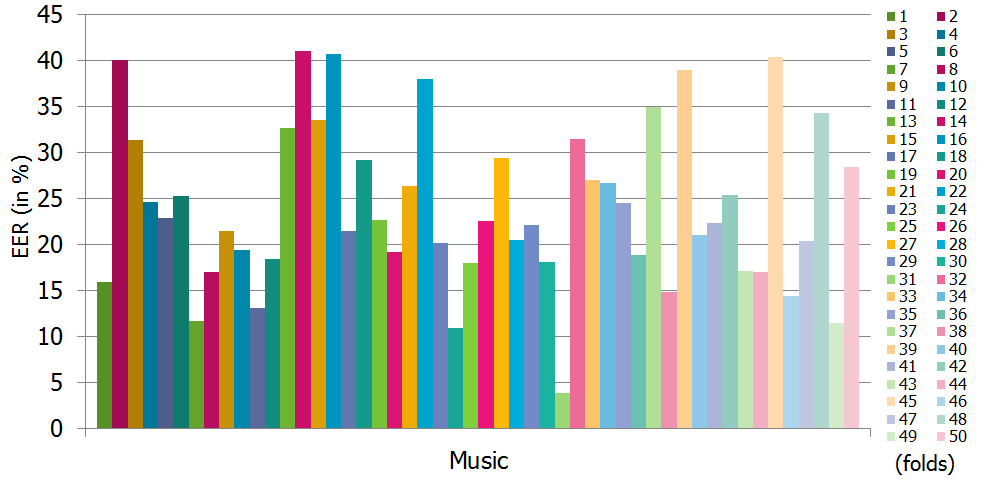
\includegraphics[width=0.9\columnwidth]{music-50CV-noaug} 
\caption['Music' model: 50-fold cross validation results]{'Music' model: 50-fold cross validation results}
\label{fig:music-50CV-noaug} 
\end{figure}

\paragraph{Overall Results Comparison: CNN vs SVM}

Table~\ref{tab:cnn_db2_overall} shows the comparison of the results of all 4 classes obtained from the different models. It can be noted that the implemented CNN model outperforms the others in all the classes except 'Music'. Interestingly, the results of the CNN model for 'Music' class are even poorer than our own implemented SVM model. The results published in \cite{kons2013audio} also show that for the 'Music' class, SVM performs better than their implemented DNN model. 

One thing is however clear that compared to the SVM results of \cite{kons2013audio}, our (SVM and CNN) results for the 'Music' class are much poorer. This is, as stated earlier, primarily due to loss of some 'Music' data from the original dataset.

\begin{table}[tb]
\caption[Results comparison: CNN and SVM]{Results comparison: CNN and SVM}
\label{tab:cnn_db2_overall}
\centering
\begin{tabular}{cccc}
\toprule
Audio Class & SVM  & SVM & CNN  \\
& (results from \cite{kons2013audio}) & (our implementation) &  \\
\midrule
Crowd	& $19.82 \pm 1.15$  & $17.45 \pm 1.08$ &  $14.86 \pm 0.86$\\
Applause	& $10.18 \pm 0.81$ & $12.87 \pm 1.07$ &  $4.87 \pm 0.44$\\
Music	& $17.77 \pm 1.15$ & $23.82 \pm 1.82$  &  $24.04 \pm 1.23$\\
Traffic	& $16.38 \pm 0.77$ & $16.88 \pm 1.22$  &  $11.77 \pm 0.72$\\
\bottomrule 
\end{tabular}
\end{table}

\subsubsection{Data Augmentation}
After applying the CNN model to the dataset that was available, we attempted to artificially augment the data in order to make the model more robust against variations in the recordings. Also, the original dataset does not have enough data samples to fully realize the potential of a CNN or DNN, hence it was a motivation to increase the amount of data.

As stated earlier, we used 6 different ways of replicating the recording with label-preserving variations: (i)Changing Pitch, (ii)Adding Echo, (iii)Reducing Noise, (iv)Adding tremolo effect, (v)Adding noise and (vi)Adding reverb. It took too long to try all the different permutations of these 6 kinds of data augmentations, hence, doing a 50-fold cross-validation experiment each time became unfeasible. So, we experimented with each of these methods only for a single split of training and validation data. Most of the CNN hyper-parameters are the same as those used in our earlier CNN experiments with this dataset. Table~\ref{tab:cnn_aug_db2} reviews briefly the set of hyper-parameters used in this experiment. 

We trained 8 networks for each of our 4 classes. The only difference between these networks was the input (training data) fed to them. The term 'original' is used hereafter to represent the original dataset that we obtained from \cite{kons2013audio}. Using the 6 above-mentioned ways of augmenting data, we created 6 more copies of our dataset by applying the 6 different kind of augmentation techniques one-by-one to the original dataset. For convenience we name these 6 new copies of dataset as: (i)'echo' - where echo is added to the original data, (ii)'noise-addition' - where noise is added to the original data, (iii)'reverb' - where reverb is added, (iv)'noise-reduction' - when noise reduction is applied to the original data, (v)'pitch' - when the pitch of original recordings is increased by 20\%, and (vi)'tremolo' - when the tremolo effect is added to the original recordings. Hence the 8 networks that we trained have the following respective input data:
(I) 'original'
(II) 'original' + 'echo'
(III) 'original' + 'noise-addition'
(IV) 'original' + 'reverb'
(V) 'original' + 'noise-reduction'
(VI) 'original' + 'pitch'
(VII) 'original' + 'tremolo'
(VIII) 'original' + 'echo' + 'noise-addition' + 'reverb' + 'noise-reduction' + 'pitch' + 'tremolo'

Figures~\ref{fig:crowd-aug},\ref{fig:traffic-aug},\ref{fig:applause-aug} and \ref{fig:music-aug} show the 8 different EER curves for each of the data augmentation model for all 4 classes: 'Crowd', 'Traffic', 'Applause' and 'Music' respectively. Note that in the figures, 'everything' refers to the case (VIII) where all the six augmented datasets along with the original dataset is fed to the CNN. Figure~\ref{fig:data_aug_overall} compares the different augmentation approaches for all 4 audio classes. While there are notable improvements in performance using for example 'noise-addition' or 'noise-reduction' for 'Applause' class, 'pitch' for 'Crowd' class, etc. but there are also cases where data augmentation doesn't help, for example in the 'Traffic' class.  

[------------------------MORE EXPLANATION NEEDED HERE-------------------------]

\begin{table}[tb]
\caption[Hyper-paramter setting: CNN with data augmentation]{Hyper-parameter setting: CNN with data augmentation}
\label{tab:cnn_aug_db2}
\centering
\begin{tabular}{ccc}
\toprule
Hyper-parameter & Value  \\
\midrule
Learning Rate	& 0.003\\
Batch Size	& 50\\
Number of epochs & 500\\
Original training samples 	& 3300\\
Validation samples & 800\\
\bottomrule 
\end{tabular}
\end{table}


\begin{figure}[!htb] 
\centering 
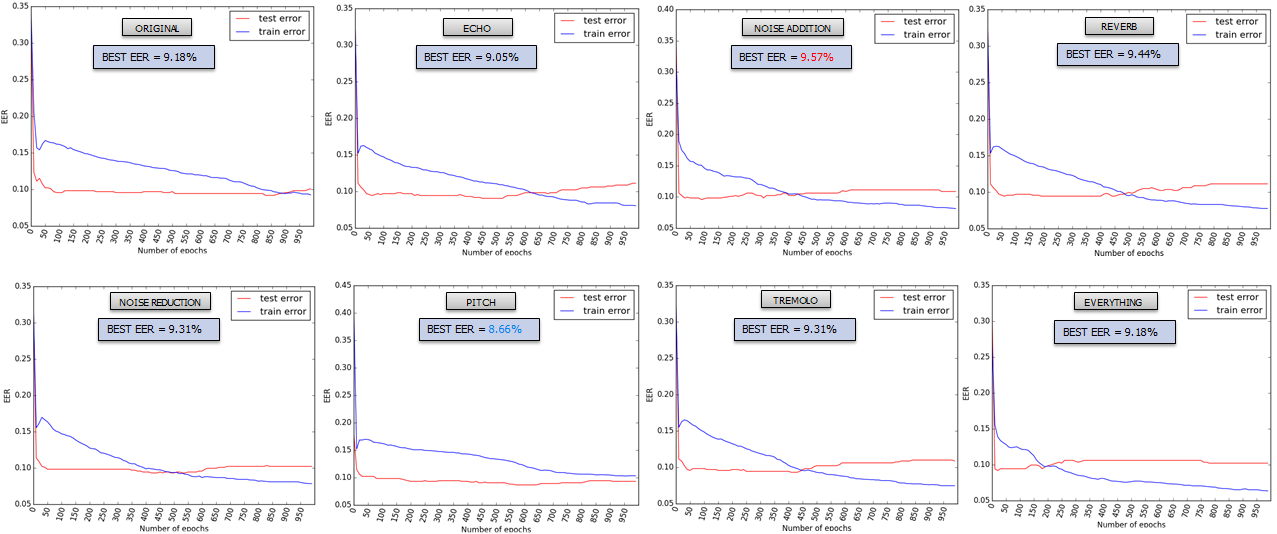
\includegraphics[width=0.95\columnwidth]{crowd-aug}
\caption[EER curves for the 8 different CNN models with data-augmentation for 'Crowd' class]{EER curves for the 8 different CNN models with data-augmentation for 'Crowd' class}
\label{fig:crowd-aug} 
\end{figure}

\begin{figure}[!htb] 
\centering 
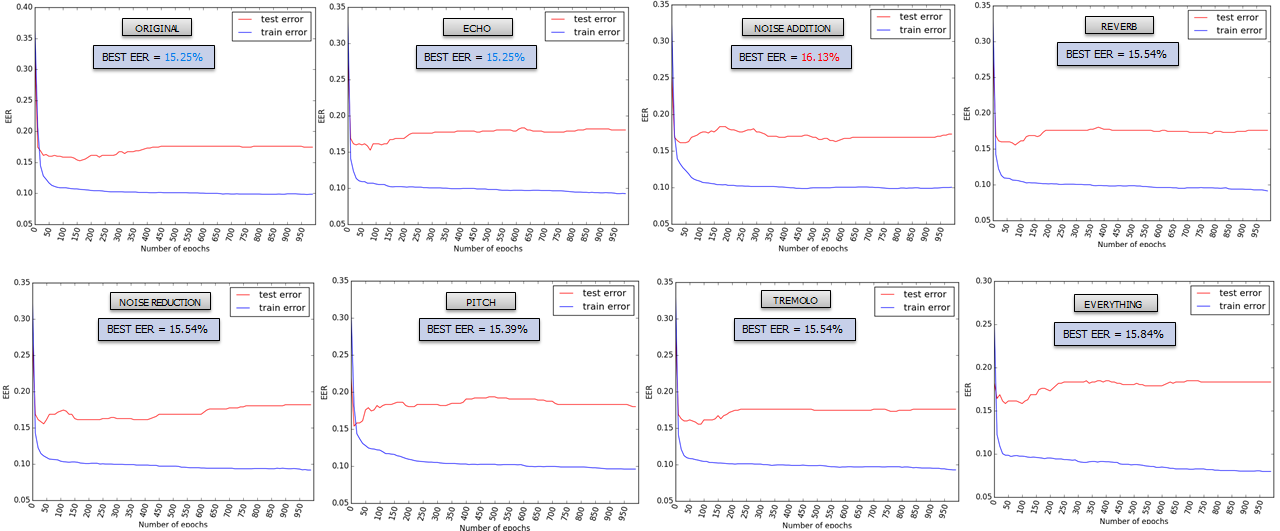
\includegraphics[width=0.95\columnwidth]{traffic-aug}
\caption[EER curves for the 8 different CNN models with data-augmentation for 'Traffic' class]{EER curves for the 8 different CNN models with data-augmentation for 'Traffic' class}
\label{fig:traffic-aug} 
\end{figure}

\begin{figure}[!htb] 
\centering 
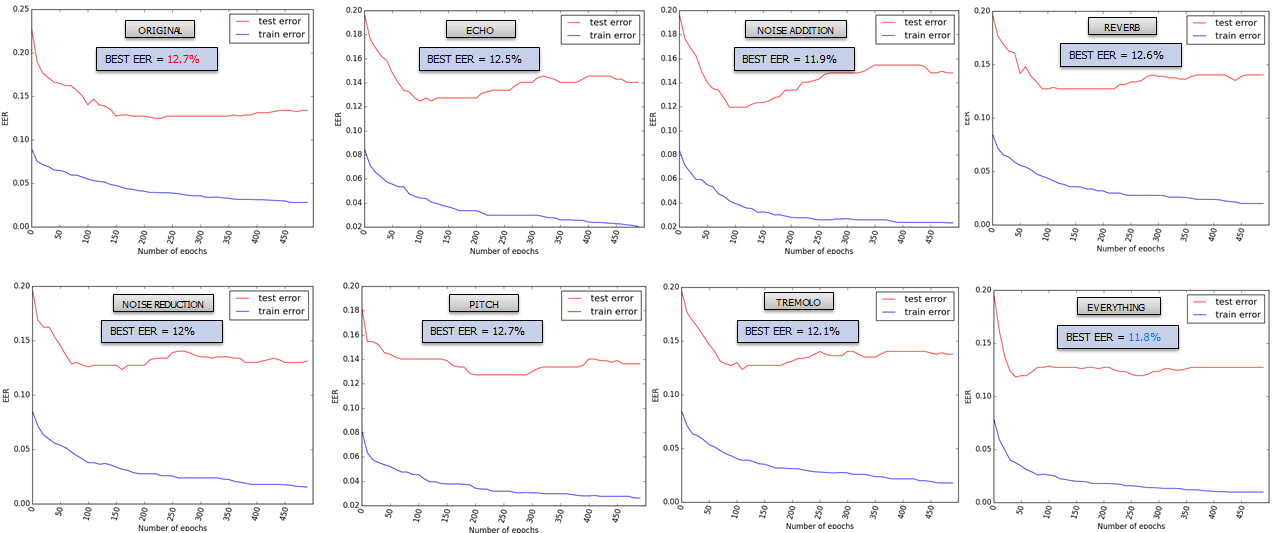
\includegraphics[width=0.95\columnwidth]{applause-aug}
\caption[EER curves for the 8 different CNN models with data-augmentation for 'Applause' class]{EER curves for the 8 different CNN models with data-augmentation for 'Applause' class}
\label{fig:applause-aug} 
\end{figure}

\begin{figure}[!htb] 
\centering 
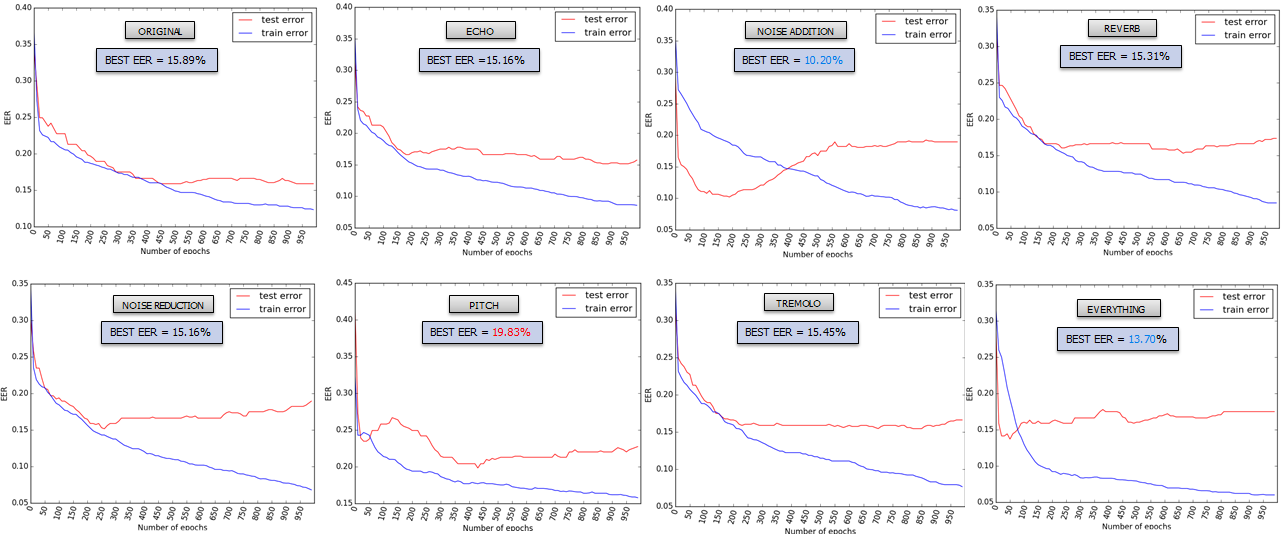
\includegraphics[width=0.95\columnwidth]{music-aug}
\caption[EER curves for the 8 different CNN models with data-augmentation for 'Music' class]{EER curves for the 8 different CNN models with data-augmentation for 'Music' class}
\label{fig:music-aug} 
\end{figure}

\begin{figure}[!htb] 
\centering 
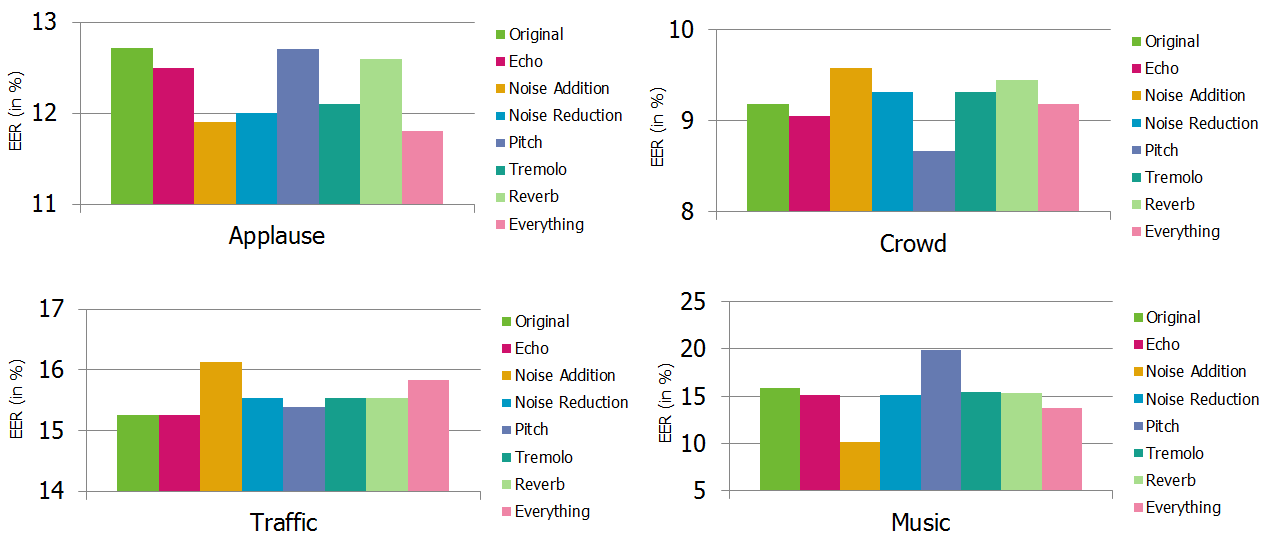
\includegraphics[width=0.95\columnwidth]{data_aug_overall}
\caption[Overall results comparing different data augmentation methods across the 4 audio classes]{Overall results comparing different data augmentation methods across the 4 audio classes}
\label{fig:data_aug_overall} 
\end{figure}


\section{Dataset-III}

The CHiME dataset is another dataset suitable for performing polyphonic audio event detection system. As discussed earlier, this dataset is composed of sounds from a domestic/home environment. The dataset comprises of 7 different audio classes which are reviewed in table~\ref{tab:audio_classes_db3}. 

First we tried to reproduce the baseline results published at \cite{foster2015chime} for this database using GMM. Then we examined the results produced by our implemented CNN model on this database. The implementation of the GMM model was completely motivated from \cite{foster2015chime}. For the CNN model, we trained 7 different one-vs-all binary classifiers, one for each class. This is similar to the approach we followed for dataset-II. 

In the following, we discuss the evaluation procedure adopted to evaluate or results on this dataset, and then we present the results of our models and compare them with the baseline results of \cite{foster2015chime}. 

\begin{table}[tb]
\caption[CHiME Dataset - Audio Classes]{CHiME Dataset - Audio Classes}
\label{tab:audio_classes_db3}
\centering
\begin{tabular}{ccc}
\toprule
Label & Description  \\
\midrule
c	& Child speech\\
m	& Adult male speech\\
f & Adult female speech\\
v 	& Video game/TV\\
p & Percussive sounds, e.g. crash, bang, knock, footsteps\\
b & Broadband noise, e.g. household appliances\\
o & Other identifiable sounds\\
\bottomrule 
\end{tabular}
\end{table}

\subsection{Evaluation Procedure}
Motivated by \cite{foster2015chime}, which is the source of this dataset, we use the AUC - area under (ROC) curve as the evaluation metric to evaluate the performance of our models. In the following we explain how the AUC is computed.

Besides EER (equal error rate), an error metric discussed in section\ref{eval_proc_db2}, AUC is another reliable metric to estimate the classification accuracy of a binary classifier where there is a class-skew between the positive and negative classes. When we train 7 different classifiers per class, the number of positive data samples is much smaller than the number of negative data samples. Hence, AUC is a promising error metric for our case.

In this dataset, the audio recordings are 4 seconds long. Each audio recording is fed as one training data instance to the classifier (CNN) which then outputs a probability. This probability indicates whether the recording belongs to the positive or the negative class depending on a high value (say 0.9) or a low value (say 0.1) respectively. The ROC curve is plotted between the \textsl{true positive rate} (TPR) and the \textsl{false positive rate} (FPR), which are computed by the comparison of the model predictions and the ground truth. (Details about ROC curve discussed in section~\ref{eval_proc_db2}). AUC is then the area under this ROC curve. The higher the area, the better the classification performance of the classifier. A purely random classifier would have an AUC score of 50\% and an ideal binary classifier would have an AUC score of 100\%. Figure~\ref{fig:auc_roc} shows the AUC for a binary classifier and a random classifier. It can be seen that the area under curve for the random classifier is 50\% as stated earlier.

Similar to \cite{foster2015chime}, we perform 10-fold cross validation, holding one out of the 10 folds of data out as the test/validation set. By doing this repeatedly 10 times for the 10 folds, we get the predictions for the 10 different folds of the test/validation data. In the end we concatenate the predictions of all these 10 folds of test data (which ultimately equals to the full dataset) and then compute the AUC by comparing these predictions to the ground truth value. This is done for each of the 7 classifiers, hence, we obtain 7 different AUC scores, one for each classifier.

\begin{figure}[!htb] 
\centering 
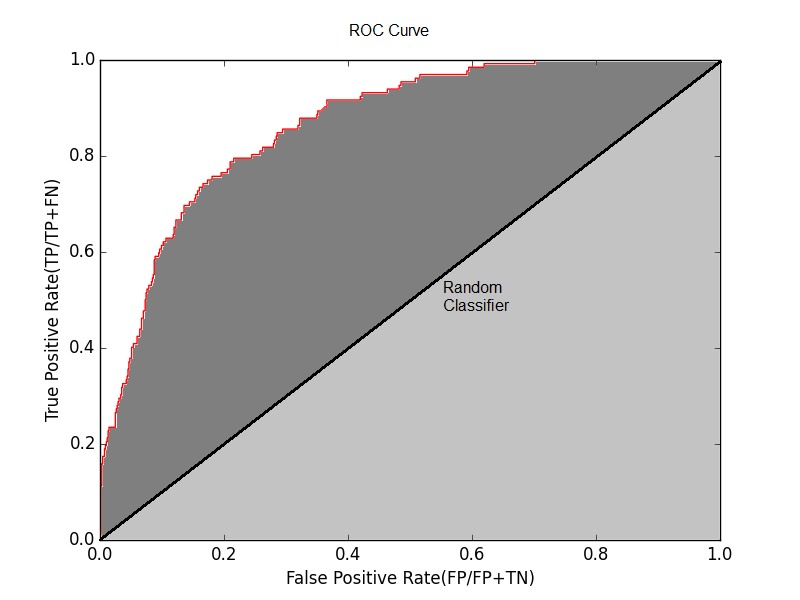
\includegraphics[width=0.95\columnwidth]{auc_roc}
\caption[Area Under ROC Curve]{Area Under ROC Curve}
\label{fig:auc_roc} 
\end{figure}


\subsection{Results}

\subsubsection{Baseline: Gaussian Mixture Models}
We develop and train the GMM models as an attempt to reproduce the baseline GMM results published in \cite{foster2015chime}. We have 7 audio classes, hence, for each class we train a pair of GMMs, one pertaining to the positive class and the other to the negative class. As  a part of the experiment, the number of Gaussians are varied using the values in the set {1,2,4,8}. We estimate full-covariance Gaussians and finally for each audio class 'c' and for each audio recording 'r', prediction is made by computing the log-likelihood ratio of the feature-vector corresponding to 'r', with respect to the pair of estimated GMMs. This prediction indicates the probability with which 'r' belongs to class 'c'.

As discussed in the previous section, we perform a 10-fold cross validation experiment for each of the 7 audio classes. The AUCs computed for each audio class are displayed in figure~\ref{fig:gmm_result_db3} along-with the baseline results of \cite{foster2015chime}. It can be seen that our GMM implementation closely reproduces the results from \cite{foster2015chime}. The next step is then to apply this dataset to our CNN model with the aim of getting better results than those obtained using GMM. 

\begin{figure}[!htb] 
\centering 
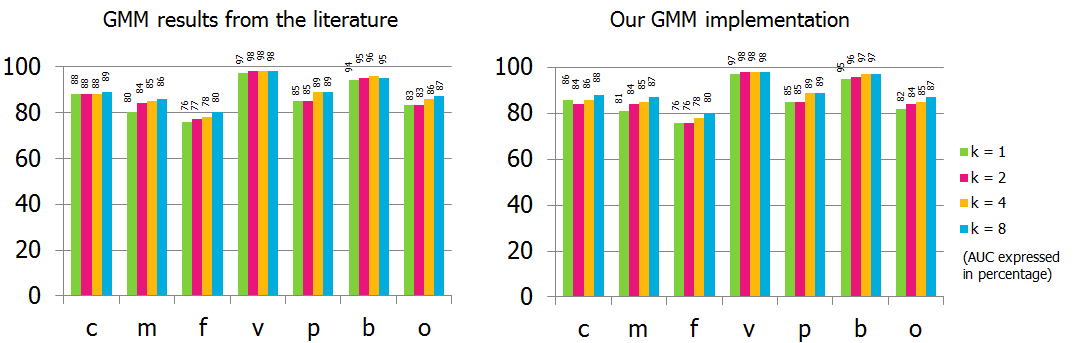
\includegraphics[width=0.95\columnwidth]{gmm_result_db3}
\caption[GMM Results: Baseline results from literature (left), and results from our implemented GMM (right)]{GMM Results: Baseline results from literature (left), and results from our implemented GMM (right)}
\label{fig:gmm_result_db3} 
\end{figure}

\subsubsection{Convolutional Neural Network}
We train 7 different CNN models, one per audio class and perform a 10-fold cross-validation experiment as done with GMM. However, we tried a grid of hyper-parameter for each of the 7 models. Basically we experimented with 16 different permutations of controllable hyper-parameters for each of the 7 models. Table~\ref{tab:hyper_param_grid_cnn_db3} shows the 16 different sets of hyper-parameters that we tried on our CNN models.

\begin{table}[tb]
\caption[Hyper-parameter grid for CNN model]{Hyper-parameter grid for CNN model}
\label{tab:hyper_param_grid_cnn_db3}
\centering
\begin{tabular}{ccccccc}
\toprule
ID & Learning Rate & Epochs & Batch-size & Output feature maps & Kernel size & Max-pool size \\
\midrule
1	& 0.01 & 500 & 50 & 7 & (7,1) & (10,1)\\
2	& 0.003 & 1000 & 50 & 7 & (7,1) & (10,1)\\
3   & 0.003 & 1000 & 100 & 7 & (7,1) & (10,1)\\
4 	& 0.03 & 500 & 20 & 7 & (7,1) &  (10,1)\\
5   & 0.001 & 1000 & 50 & 7 & (7,1) & (10,1)\\
6   & 0.01 & 500 & 50 & 26 & (7,1) &  (10,1)\\
7   & 0.01 & 500 & 50 & 15 & (7,1) &  (10,1)\\
8   & 0.01 & 500 & 50 & 7 & (5,1) &  (12,1)\\
9   & 0.01 & 500 & 50 & 7 & (9,1) & (8,1)\\
10   & 0.01 & 500 & 50 & 15 & (5,1) & (12,1)\\
11   & 0.01 & 500 & 50 & 4 & (9,1) & (8,1)\\
12   & 0.001 & 1000 & 50 & 26 & (14,1) & (11,1)\\
13   & 0.001 & 1000 & 50 & 10 & (3,1) & (11,1)\\
14   & 0.01 & 500 & 50 & 7 & (3,1) &  (11,1)\\
15   & 0.01 & 500 & 50 & 5 & (3,1) & (17,1)\\
16   & 0.01 & 500 & 50 & 13 & (17,1) & (18,1)\\
\bottomrule 
\end{tabular}
\end{table}

We tried these 16 different permutations of hyper-parameters on each of the 7 CNN models. Table~\ref{tab:cnn_result_db3} shows the best AUC performance (in \%) obtained from these CNN models along with the permutation IDs, which tells the sets of hyper-parameters that give those best CNN results. We also compare these results with the best GMM baseline results (from literature) for each of the 7 classes.

[HERE ON, SHOW IMPROVEMENT IN CNN RESULTS BY e.g. TRANSFER LEARNING, etc.]

\begin{table}[tb]
\caption[CNN results in comparison with the best GMM results]{CNN results in comparison with the best GMM results}
\label{tab:cnn_result_db3}
\centering
\begin{tabular}{cccc}
\toprule
Class label & Best GMM result & Best CNN result & Permutation IDs  \\
\midrule
c & 89 & 89 & (8,16)\\
m & 86 & 81 & (6,7,8,10,16)\\
f & 80 & 77 & (15,16)\\
v & 98 & 99 & (1,2,4)\\
p & 89 & 87 & (15,16)\\
b & 96 & 97 & (9,14,15)\\
o & 87 & 84 & (16)\\
\bottomrule 
\end{tabular}
\end{table}